\documentclass[11pt, a4paper, titlepage]{article}
\usepackage[onehalfspacing]{setspace} 
\usepackage{fullpage}
\usepackage{helvet}
\renewcommand{\familydefault}{\sfdefault}
\usepackage{graphicx}
\graphicspath{./images/}
\usepackage{float} % needed for [H]
\usepackage{titlesec}
\usepackage{lineno}
\usepackage[round]{natbib}
\usepackage[margin=2cm]{geometry}
\usepackage{hyperref}
\usepackage{caption} % So that i can position figures
\usepackage[labelfont=bf,textfont=bf]{caption} % Makes figure title bold
\hypersetup{
	colorlinks,
	linkcolor={black!50!black}, %colour of contents links
	citecolor={blue!50!black},
	urlcolor={blue!80!black}
}
\linenumbers
\onehalfspacing
\usepackage{pgfgantt}


\begin{document}
    \begin{titlepage}
    \begin{center}
            {\large IMPERIAL COLLEGE LONDON}
    \end{center}
    
    \vspace*{\fill}
    
    \begin{center}
        {\Huge 
    	 Geographical Variations in the Sensitivity of Terrestrial Biodiversity to Anthropogenic Pressures}
        \\[2in]
        Author: Kayleigh Greenwood, MSc CMEE (kg21@ic.ac.uk)
        \bigskip
        \newline
       Internal Supervisor: Dr James Rosindell, Imperial College London (j.rosindell@imperial.ac.uk)
       \bigskip
       \newline
        External Supervisor: Dr Joss Wright, University of Oxford (joss.wright@oii.ox.ac.uk)
        \bigskip
        \newline

        25/08/2022
        \\[2in]
        
        {\bfseries A thesis submitted in partial fulfilment of the requirements for the degree of Master of Science at Imperial College London \newline \newline Submitted for the MSc in Computational Methods in Ecology and Evolution }

        

    
	\end{center}
    \vspace{\fill}
    
    \end{titlepage}
	\section*{Declaration}
	\begin{center}
	Data was obtained from existing online databases, and therefore I was not responsible for data processing or cleaning. \newline
	Were any mathematical models developed by you or by your supervisor? \newline
	What role, if any, did your supervisor play in developing the analyses presented?
	\end{center}
	\newpage
	
	\section*{Abstract}
	 To our knowledge, very little prior research has studied geographic differences in sensitivity to biodiversity pressures. Hence, studying geographical variation in  sensitivity would be useful in comparing the impact of pressures on global biodiversity.
	
\newpage
\tableofcontents
\newpage
	
    \section*{Introduction}
    \addcontentsline{toc}{section}{Introduction}
    	
    %Para 1: biodiversity is important. pressures act on biodiversity
Ecosystems with intact biodiversity provide services such as clean air and pollination, which make the earth habitable for humans \citep{leemans2003millennium}. Biodiversity loss diminishes ecosystem productivity \citep{duffy2017biodiversity} and threatens all life on earth, including human well-being \citep{diaz2006biodiversity} leading to unstable environments which are less resistant to change. Both natural and anthropogenic pressures act on biodiversity \citep{nobel2020anthropogenic}, but it it is the latter which is accelerating extinction rates dramatically \citep{ceballos2015accelerated}. Understanding the impacts of anthropogenic pressures on biodiversity is necessary to inform more effective policies, strategies and tools \citep{diaz2006biodiversity}. This understanding is aided by an understanding of the  distribution of biodiversity, how its pressures are distributed, and understanding how sensitive biodiversity is to these pressures. The worlds' biodiversity is not equally distributed, it varies geographically \citep{gaston2000global, ricklefs2004comprehensive, mcrae2017diversity}  as do the pressures acting on it \citep{millennium2005ecosystems, sala2000global, bowler2020mapping}, and these distributions often correlate \citep{ament2019compatibility, Velde2022}. Despite any such correlations between biodiversity and its pressures, there will always be variation in biodiversity response to such pressures due to variations in sensitivity of species \citep{bowler2020mapping}. \newline
   	
   	\subsection*{Interspecific Variation in Sensitivity}
   	\addcontentsline{toc}{subsection}{Interspecific Variation in Sensitivity} 
   	 %Para: Introducing species varying sensitivities and why they aren't enough
   	 Interspecific variation exists in response to biodiversity pressures \citep{foden2013identifying}. Given that both species and higher taxa \citep{sunday2015species} have shown variations in sensitivity, and each region of the world comprises different combinations of species groups \citep{goethem2021biodiversity}, there is reason to believe that sensitivity to biodiversity pressure varies depending on location. Despite this, geographical variation in sensitivity is rarely accounted for \citep{newbold2020tropical, sala2000global}. \cite{newbold2020tropical} stated that by including the sensitivity of individual species, distribution models implicitly capture geographical variation of sensitivity, but rarely explicitly include geographical variation in sensitivity. To the best of my knowledge there is no research to support this exclusion of geographical variation in sensitivity. An understanding of the sensitivity of biodiversity of an entire region could be a more accurate metric for studies of a broad scale. \newline
   	 
   	 \subsection*{Sensitivity Variation at Broader Levels}
   	 \addcontentsline{toc}{subsection}{Sensitivity Variation at Broader Levels} 
   	 Biodiversity sensitivity varies at broader levels than species and higher taxon, such as biomes and regions (discussed below), further supporting the concept that sensitivity variation could exist at levels as broad as continent. Biodiversity sensitivity differs between biomes for the following biodiversity pressures; pollution (nitrogen exceedance) \citep{alkemade2009globio3}, land use change and climate change \citep{newbold2020tropical}. The most sensitive biomes were tropical biomes \citep{barlow2016anthropogenic} with the least sensitive being temperate and boreal biomes \citep{newbold2020tropical, cazalis2021mismatch, barlow2016anthropogenic}. Despite geographical variations in sensitivity existing between biomes, little is known about continental differences. Biomes are unequally distributed between the continents, with South America having a higher percentage cover of tropical forest than any other continent, and Europe having the lowest closely followed by North America \citep{wade2003distribution}.  Because of the aforementioned sensitivity differences between biomes, it could be that Europe and North America will have lower sensitivity to biodiversity pressures than other continents, with South America being the most sensitive. However, of the minimal research that has studied continental differences, findings showed tropical forest biodiversity sensitivity to be higher in Asia than in other regions (Americas and Africa) \citep{gibson2011primary}. Despite the apparent contradiction with the above prediction (South America being the most sensitive), it must be noted that it was only Asia's tropical biome that was shown to be the highest among continents, not the biodiversity of the continent on the whole, and also not all continents were considered. \newline
   	 
   	 One of the papers which studied interspecific sensitivity to environmental pressures of European species \citep{louette2010bioscore}, suggested country-level differences in sensitivity variation. Using species distribution data, the proportion of sensitive species in each country was used to map the effects of a change in each biodiversity pressure on the biodiversity of Europe. The tool (`Bioscore') produces a map of impact across Europe in response to changes in each of the biodiversity pressures, which suggests that even if the magnitude of a biodiversity pressure is constant across Europe, biodiversity response can still vary according to country, due to varying sensitivity of the species within such country. Though the map produced by the tool appears to show variations in sensitivity between countries, the tool is outdated and the data and code are inaccessible, with no values for country level sensitivities having been published. The BioScore tool's predictions support the concept that country-wide differences in sensitivity could exist, however an up to date, wider-breadth study is necessary to observe worldwide variances in countries sensitivities to biodiversity pressures. \newline
   	 

   	\subsection*{Knowledge Gap}
   	\addcontentsline{toc}{subsection}{Reason for gap in knowledge} 
 	A possible explanation for the inadequate research on sensitivity distribution is that sensitivity studies typically use a method of determining the sensitivity of individual species (obtained from published literature about individual species' responses to change), and then mapping these sensitivity values to look for trends \citep{louette2010bioscore}. Because of the intensity of this method, and the under-representation of certain regions \citep{collen2008tropical}, a global sensitivity analysis looking at regional biodiversity sensitivity would be very labour-intense. Additionally, most distribution studies focus on the most important pressures \citep{ferrier2016summary}. This study aims to use an alternate method, as described further below, using biodiversity and pressure trends at the regional level to look for geographic patterns in sensitivity to the five main biodiversity pressures (climate change, land use change, pollution, overexploitation and invasive species). Having regional information on biodiversity sensitivity will allow the impact of pressures on biodiversity to be better estimated in situations where it is not clear which species are being impacted, and only the area of impact is known. Rather than just including how biodiversity in general is likely to respond, it would be more useful to know how local biodiversity in that specific region is likely to respond.  \newline
   	 

   	
   	\subsection*{Research aims}
   	\addcontentsline{toc}{subsection}{Research aims}
   	
   	%Para: Conclusion
   	 Given that anthropogenic impact on the environment is worldwide \citep{plumptre2021might}, the question should be raised of whether the geographic location of biodiversity pressures affects their impact on global biodiversity. The understanding of variations in biodiversity sensitivity, along with many other aspects of biodiversity, has knowledge gaps which desperately need filling \citep{pereira2012global}. If such geographic differences exist, they should be taken into account when attributing biodiversity-related merit to investments. To widen the scope of impact outside of the Benchmark for Nature project, taking into account geographic variations in sensitivity to biodiversity pressures could make estimates about biodiversity impact more accurate. Better understanding of biodiversity pressures will aid a better understanding of the implications of investments (and other policies) on natural ecosystems.
   	 
   	%para: aims
 	The aim of this project is to investigate whether sensitivity of biodiversity to pressures varies geographically. I will amalgamate country-level data to look at continental differences in the main pressures on biodiversity. I hypothesise that continents with a higher proportion of tropical biomes (e.g. South America) will have higher sensitivity scores than continents with a lower proportion of tropical biomes (e.g Europe and North America) across all pressures.  \newpage

    \section*{Methods}
	\addcontentsline{toc}{section}{Methods}
	 % very very very important that if i'm using BII, i talk about measuring biodiversity INTACTNESS instead of measuring biodiversity.
	\subsection*{Overview}
	\addcontentsline{toc}{subsection}{Overview}

	The focus of this study is on anthropogenic biodiversity pressures only. Anthropogenic pressures on biodiversity are typically grouped, in the current literature, into 5 main pressures; climate change, land use change, pollution, invasive species and overexploitation \citep{watson2019summary}. In order to assess whether sensitivity to each pressure varies by country, data was needed in the form of time series (how each of these pressures had been changing in each country over time, as well as how each country's biodiversity had been changing over time). The time series of biodiversity in a country was compared to the time series of a pressure on biodiversity in that country, in order to extract a `sensitivity score' for each country to assess any effect of geography. Due to comparisons between countries, only terrestrial biodiversity was included. \newline
	% Get James' opinion
	
	First, each pressure's geographic relationship with biodiversity was assessed in isolation. It is important to look at individual biodiversity pressures, as opposed to an aggregated pressure on biodiversity, because the pressures have spatial differences \citep{steffen2015planetary}, meaning the geographical magnitude of each pressure varies. Therefore in order to understand how countries differ in their responses to biodiversity pressures, it must be taken into account the magnitude of each pressure that each country experiences. \newline
	
	I used linear models on time series data about biodiversity and its five main pressures at the country level, and interpret the gradient coefficients as the sensitivity' of that country's biodiversity to each pressure. I will further analyse these sensitivity scores to look for geographic variation in sensitivity between the continents. In comparison to the previously mentioned common method of gathering information about species-level sensitivities and mapping them, this method is less labour intense and is designed to give broad insights into whether biodiversity trends differ among continents. \newline
	% get James' opinion
	\subsection*{Data}
	\addcontentsline{toc}{subsection}{Data}
	
	% BD data = 18 years, 240 countries
	The variable chosen to represent biodiversity was biodiversity intactness. The National History Museum's (NHM) Biodiversity Intactness Index (BII)\citep{phillips2021} was chosen as it presents biodiversity in the context of how many original species remain (relative to reference populations). The NHM's Index is the best for this project as the database used is that of the PREDICTS project, which more geographically representative than other datasets \citep{purvis2018modelling}. This allows for direct comparison of these changes, with the changes in anthropogenic pressures. Historical BII data spanned 18 years between 1970 - 2014. \newline
	
	% Climate data = 230 countries
	Time series data for climate change was obtained in the form of annual average temperature for each country. The temperature dataset chosen was from the World Bank's Climate Change Knowledge Portal. This dataset was chosen because it contains comprehensive historical data, providing an annual average temperature for every year from 1900 until 2020. \newline
	
	% Built Land data = 249 countries (years is big problem!) \newline
	To represent land use change, the dataset used was The Global Human Settlement Layer data package \citep{JRC117104}. The data contains information on built-up area change over time, which is the variable chosen to represent land use change. Collective land use change is difficult to quantify from land use statistics. Although satellite data is available to categorise land cover type over time, calculating annual land use change from the proportion of each land cover type is not necessarily accurate, as land use change can be multi-directional. Current studies assessing the impact of land use change on biodiversity are often meta-analyses or use a natural regional situation as the reference land type \citep{de2013land} as opposed to observing direct impacts of land use change. A limitation of this dataset is that only 4 years of data are included. \newline
	
	% GHG data = 31 years, 63 countries (countries is problem!) \newline
	With the focus being on terrestrial biodiversity, greenhouse gases (GHG) were used as the representative variable for `pollution' as a biodiversity pressure. The dataset used to access GHG emissions for each country over time was the `National Inventory Submissions' section of the United Nations - Climate Change website \citep{united nations}. GHG emissions are presented both including and excluding `Land Use, Land-Use Change and Forestry (LULUCF)' related emissions data. When assessing pollution and biodiversity links in isolation, LULUCF was included. However, when modelling all biodiversity pressures together, LULUCF was tested for collinearity with the land use change variable, and consequently included/excluded. \newline
	
	The OECD.stat website was used to download the land use change and pollution data. \newline
	
	Overexploitation was excluded for multiple reasons. Firstly, overexploitation is the vaguest of the main pressures, and is usually used in the context of fishing (marine biodiversity being beyond the scope of this project). One of the most relevant aspects of overexploitation to is deforestation, which is (maybe remove this part depending on methods) already represented in the variable used for land use change. Though there are other aspects of overexploitation that would be relevant (e.g. illegal wildlife trading), there are no databases/studies available representing overexploitation by country.



	\subsection*{Individual Pressure Models}
	\addcontentsline{toc}{subsection}{Individual Pressures}
	
	\subsection*{Data Wrangling}
	\addcontentsline{toc}{subsection}{Data Wrangling} 
	
	Each data set has data from a different combination of years, and countries. For each pressure being investigated, only data from years and countries that are shared between that particular dataset and the biodiversity dataset is included. \newline
	
	For each pressure, the datasets were wrangled and refined to obtain two time series (at an annual level) for each country; biodiversity and the magnitude of the particular pressure.
	
	\subsection*{Modelling}
	\addcontentsline{toc}{subsection}{Modelling} 
	
	For each country, a linear model was fit with biodiversity as the response variable, and the biodiversity pressure (e.g. pollution) as the explanatory variable. The gradient coefficient was recorded as a `sensitivity score', with the standard error of the gradient also recorded, for use in the next step. This sensitivity score is representative of the sensitivity of that country's biodiversity, to the particular biodiversity pressure (e.g., sensitivity of a country's biodiversity to one unit of pollution). The unit of sensitivity scores depend on the pressure being modelled, and represent the change in Biodiversity Intactness Index (BII) for a unit increase in pressure. \newline
	

	Sensitivity scores were then compared between continents using a linear model. The weights function of lm() was used to take account for the standard errors of the gradients from the first step, and the inverse of the standard errors were inputted as weights (weights in lm() is inversely proportional to variance). Important to note that this method only tests for differences between each category, and the reference category, and therefore does not test differences between all groups.  \newline
	
	
	\subsection*{Multi-Pressure Model}
	\addcontentsline{toc}{subsection}{Multi-pressure model}
		
	\subsection*{Data Wrangling}
	\addcontentsline{toc}{subsection}{Data Wrangling} 
	The data for all countries was pooled into one dataset, and a column added for continent. Because assessing differences between each country would remove too many degrees of freedom, differences between the sensitivities of continents were assessed.
	 
	\subsection*{Modelling}
	\addcontentsline{toc}{subsection}{Modelling} 
	
	A multiple linear model was created for each pressure. Continent was coded as a factor, in order for R to treat it as a dummy variable. The alphabetically first continent acting as the reference variable (usually Africa), in order to avoid multicollinearity. So that the slopes of each continent could be compared, interactions were also added between continent and the climate \newline


	

	
	
	\subsection*{Benchmark data}
	\addcontentsline{toc}{subsection}{Benchmark data}
		
	`Benchmark for Nature' is a project which is using open-source data from news articles that have been web-scraped, in an effort to gain the maximum amount of data possible about the links that companies/sectors have with each biodiversity pressure.
	The purpose of the project is to better inform investors so that more biodiversity-conscious decisions can be made, in an effort to aid the biodiversity loss crisis \citep{gasu2021review}, and also indirectly, the climate \citep{shin2022actions}.
	
	In order to find out which level of sensitivity insight would be useful (e.g. region and continent), I will assess the dataset already collected by the Benchmark project to determine the most commonly mentioned (and therefore most useful) location terminology in articles, in the context of biodiversity.
	
	
	
	

	\clearpage

	\section*{Results}
	\addcontentsline{toc}{section}{Results}
	 
	\subsection*{Climate Model}
	\addcontentsline{toc}{subsection}{Climate Model}
	
	158 countries and 18 years matched between the climate and biodiversity datasets. Figure 1 shows the distribution of country-level climate sensitivity scores, and Figure 2 groups them by continent. \newline

	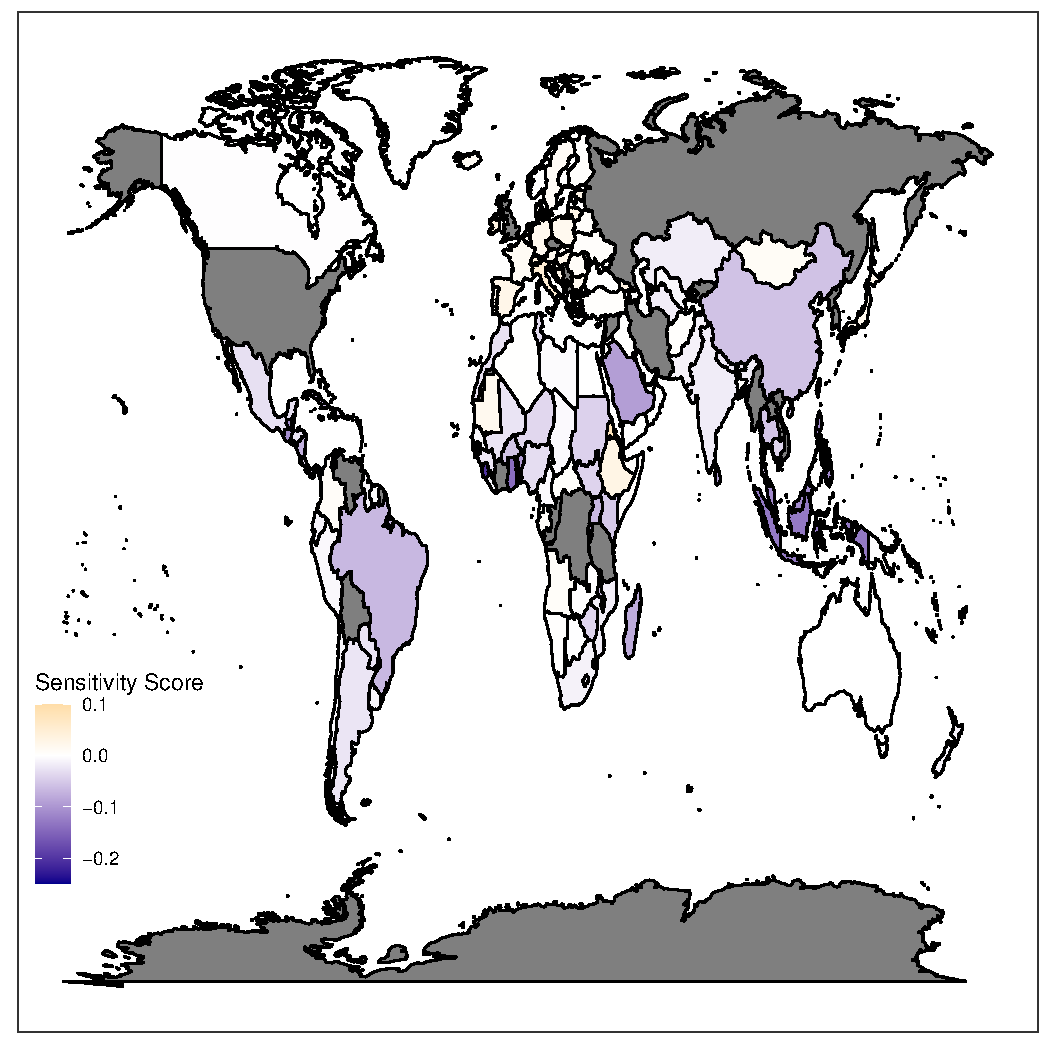
\includegraphics[scale=0.95]{../images/climatesensitivitymapgradient.pdf}
	\captionof{figure}{Biodiversity sensitivity to climate change: distribution of country sensitivity scores.}

	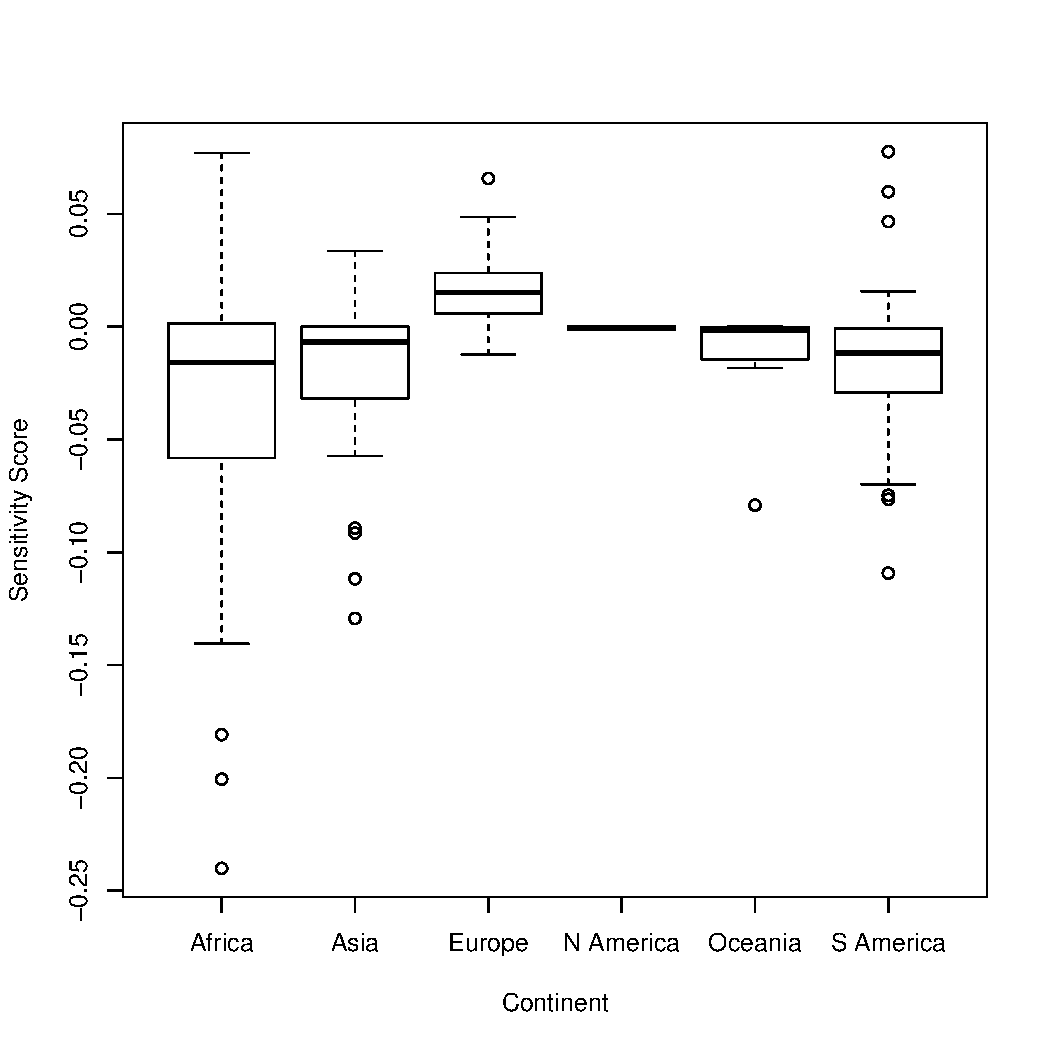
\includegraphics[scale=0.95]{../images/climatesensitivityboxplot.pdf}
	\captionof{figure}{Biodiversity sensitivity to climate change: country sensitivity scores grouped by continent.}
	\bigskip
	Africa (the reference category) was not significantly different from zero, and no other continents were significantly different from Africa apart from Europe. European countries had sensitivity scores, on average, 0.0081 higher than other continents. So for every $1^\circ C$ increase in annual temperature, the BII of countries within Europe will decrease by 0.0081 less than in other continents. 
	% Ask James to check. Would it be right to say Africas mean? 
	
	
	\newpage
	\subsection*{Pollution Model}
	\addcontentsline{toc}{subsection}{Pollution Model}
	
	There were only 43 countries and 16 years that matched between the datasets. \newline
	
	Figure 3 shows the distribution of country-level pollution sensitivity scores, and Figure 4 groups them by continent. \newline
	
	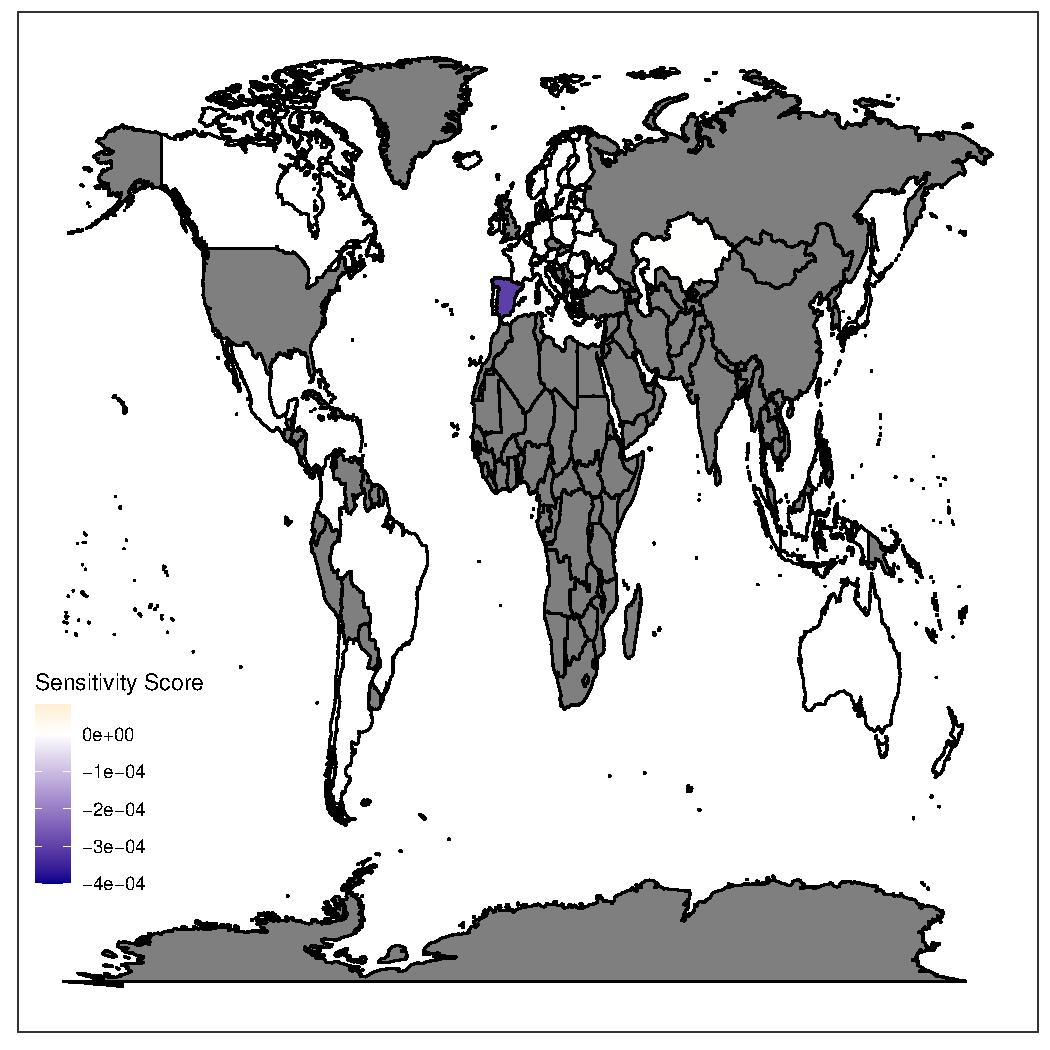
\includegraphics[scale=0.95]{../images/pollutionsensitivitymapgradient.pdf}
	\captionof{figure}{Biodiversity sensitivity to pollution.}
	
	\subsection*{Land Use Model}
	\addcontentsline{toc}{subsection}{Land Use Model}
	Built Land \newline
	
	175 countries and 3 years matched between datasets. only 1 country gave significant result.
	
	Figure 3 shows the distribution of country-level build up land sensitivity scores. \newline
	
	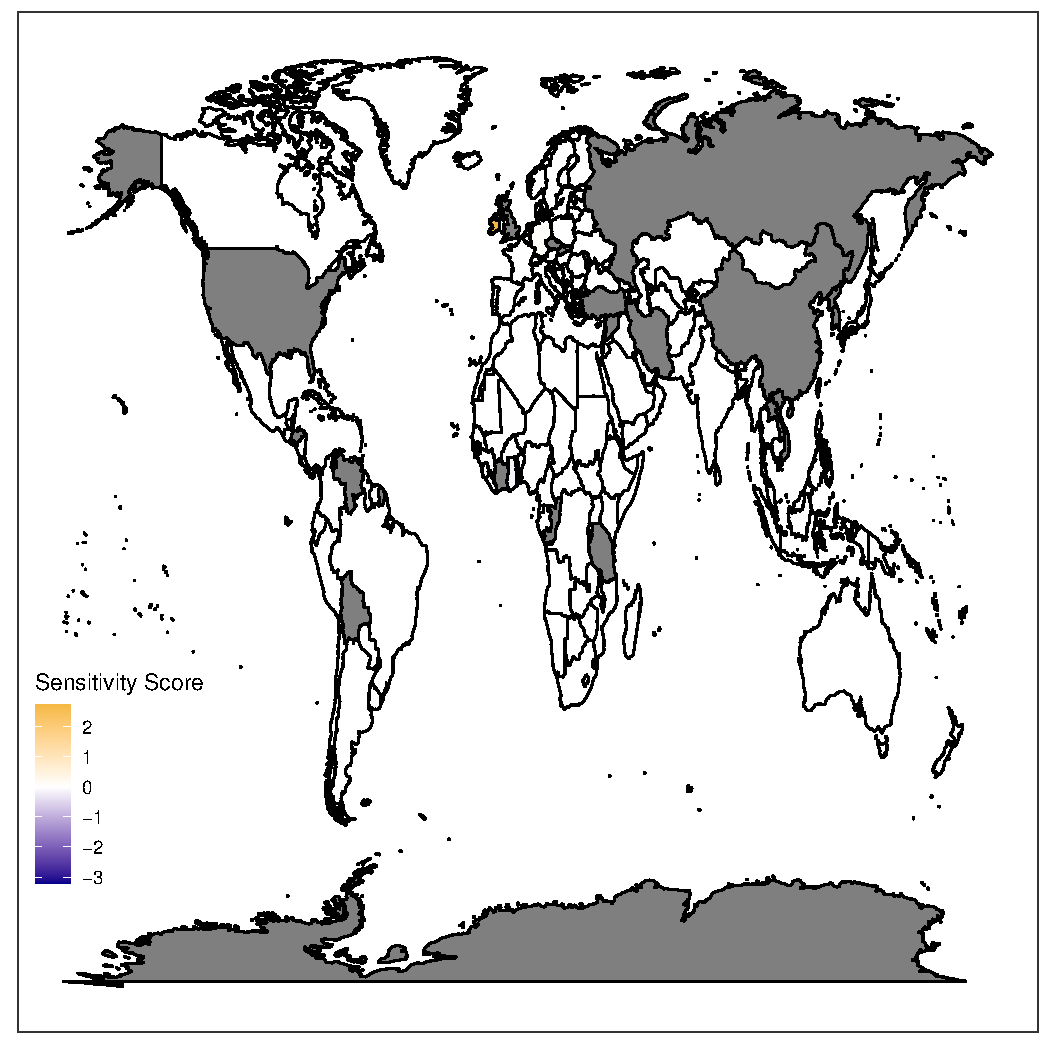
\includegraphics[scale=0.95]{../images/buildlandsensitivitymapgradient.pdf}
	\captionof{figure}{Biodiversity sensitivity to build up land.}

	\subsection*{Invasive Species Model}
	\addcontentsline{toc}{subsection}{Invasive Species Model}
	Invasive \newline
	
	147 countries matched between datasets 
	
	Figure 4 shows the distribution of country-level invasive species sensitivity scores. \newline
	
	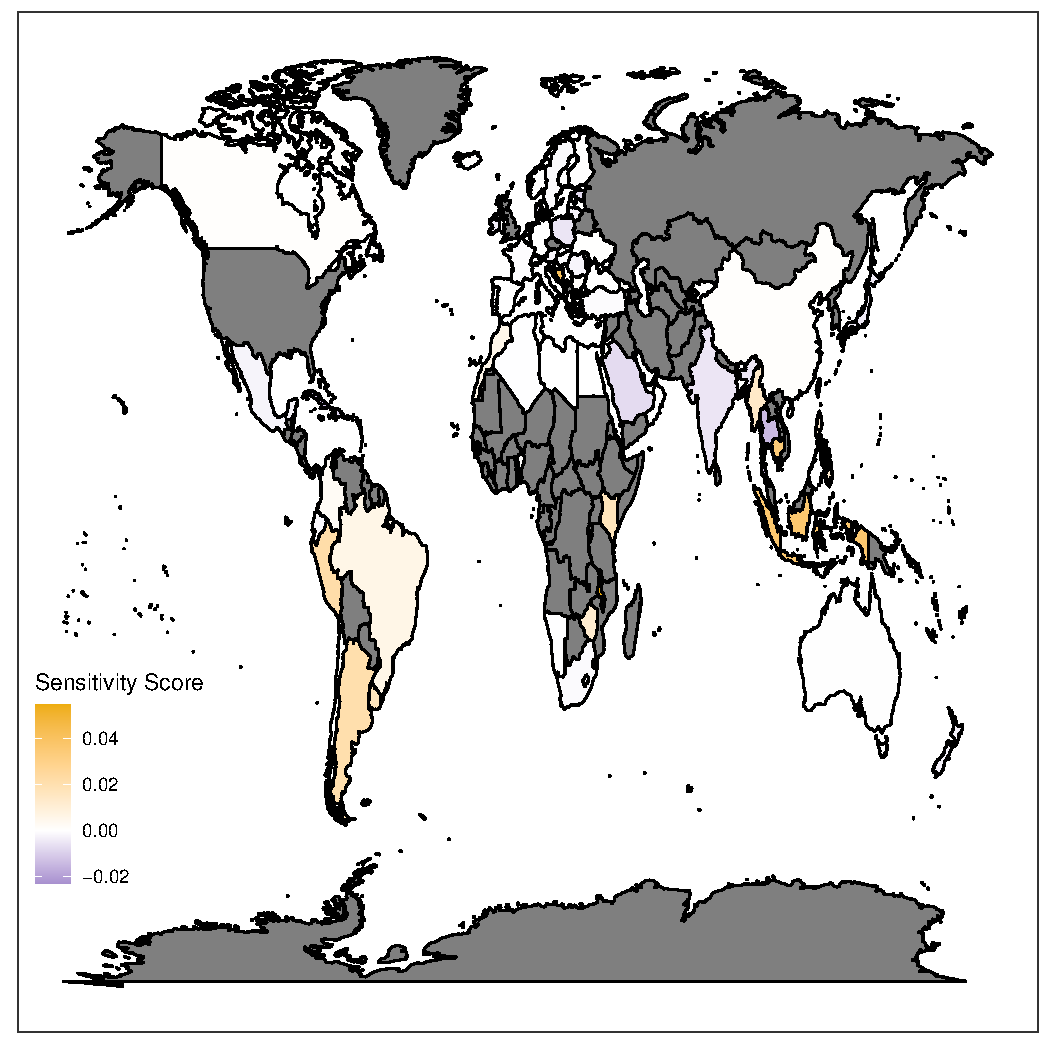
\includegraphics[scale=0.95]{../images/invasivesensitivitymapgradient.pdf}
	\captionof{figure}{Biodiversity sensitivity to Invasive species.}
	

    \clearpage
    
    
    
     \section*{Discussion}
     \addcontentsline{toc}{section}{Discussion}
     
     \subsection*{Importance of Findings}
     \addcontentsline{toc}{subsection}{Importance of Findings}
     %Para: Sustainable business and investments
     Whilst the conservation movement does a lot to help biodiversity \citep{sandbrook2019global}, another response to the biodiversity crisis \citep{ogar2020science} is the beginning of a global movement towards sustainable business and biodiversity-conscious investment \citep{pri2020, worldeconomicforum2020, wwf2020}. Creating a tool which assesses the overall biodiversity impact of a company can help guide investors, and is something that various parties are currently developing \citep{worldbenchmarkingalliance_2022, iccs_2020}.  `Benchmark for Nature' is a project which aims to use data science and to develop a framework for assessing investment impacts on biodiversity by gathering information from online articles about how much of an impact a company/sector is having on biodiversity pressures\citep{iccs_2020}, and where in the world these pressures are taking place. \newline
     \clearpage
     
     \section*{Conclusion }
     \addcontentsline{toc}{section}{Conclusion}
     optional section
     \clearpage
    
    \section*{Data and Code Availability}
    \addcontentsline{toc}{section}{Data and Code Availability}
    Data  and  CodeAvailabilitystatement:  At  the  end  of  your  Main  text,  before  the  References section, you must provide a statement titled “Data and Code Availability”, where you name a data (e.g., Dropbox, FigShare, Zenodo, etc) and a code (e.g., Dropbox, GitHub, etc.) archive 
    20from where the data and code can be obtained that will allow replication of your results. The code may be in the form of a single script file.
    
    \clearpage
    \section*{Acknowledgements}
    \addcontentsline{toc}{section}{Acknowledgements}
    \bibliographystyle{apalike}

    \bibliography{writeup}
\end{document}